\documentclass{standalone}
\usepackage{pgfplots}
\usepackage{pgfplotstable}
\pgfplotsset{compat=1.16}

\begin{document}
    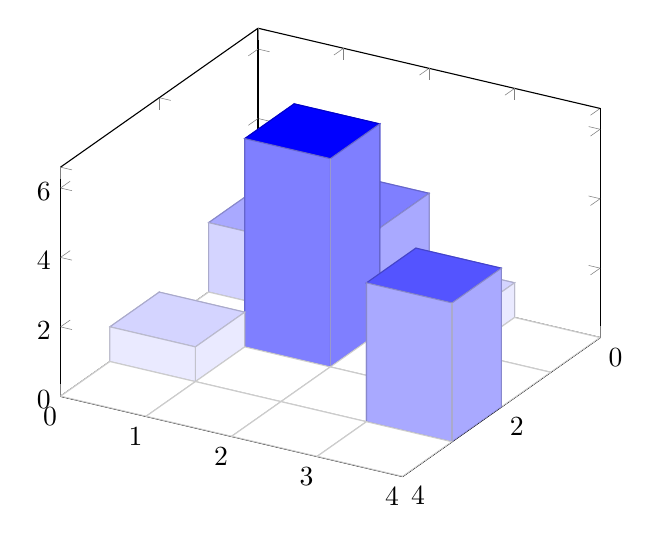
\begin{tikzpicture}
        \begin{axis}[
        view = {120}{35},% important to draw x,y in increasing order
        xmin = 0,
        ymin = 0,
        xmax = 4,
        ymax = 4,
        zmin = 0,
        unbounded coords = jump,
        colormap={pos}{color(0cm)=(white); color(6cm)=(blue)}
        ]
        \addplot3[surf,mark=none] coordinates {
            (0,0,0.0) (0,0,0.0) (0,1,0.0) (0,1,0.0) (0,2,0.0) (0,2,0.0) (0,3,0.0) (0,3,0.0) (0,4,0.0) (0,4,0.0)

            (0,0,0.0) (0,0,2) (0,1,2) (0,1,3) (0,2,3) (0,2,1) (0,3,1) (0,3,0) (0,4,0) (0,4,0.0) (1,0,0.0)

            (1,0,2) (1,1,2) (1,1,3) (1,2,3) (1,2,1) (1,3,1) (1,3,0) (1,4,0) (1,4,0.0)

            (1,0,0.0) (1,0,0) (1,1,0) (1,1,6) (1,2,6) (1,2,0) (1,3,0) (1,3,0) (1,4,0) (1,4,0.0) (2,0,0.0)

            (2,0,0) (2,1,0) (2,1,6) (2,2,6) (2,2,0) (2,3,0) (2,3,0) (2,4,0) (2,4,0.0)

            (2,0,0.0) (2,0,1) (2,1,1) (2,1,0) (2,2,0) (2,2,0) (2,3,0) (2,3,4) (2,4,4) (2,4,0.0) (3,0,0.0)

            (3,0,1) (3,1,1) (3,1,0) (3,2,0) (3,2,0) (3,3,0) (3,3,4) (3,4,4) (3,4,0.0)

            (3,0,0.0) (3,0,0) (3,1,0) (3,1,0) (3,2,0) (3,2,0) (3,3,0) (3,3,0) (3,4,0) (3,4,0.0) (4,0,0.0)

            (4,0,0) (4,1,0) (4,1,0) (4,2,0) (4,2,0) (4,3,0) (4,3,0) (4,4,0) (4,4,0.0)

            (4,0,0.0) (4,0,0.0) (4,1,0.0) (4,1,0.0) (4,2,0.0) (4,2,0.0) (4,3,0.0) (4,3,0.0) (4,4,0.0) (4,4,0.0)
        };
        \end{axis}
    \end{tikzpicture}
\end{document}